\section{Testing Methodologies}\label{sec:methodology}

We describe two types of OpenCL testing using our approach. The first is a direct comparison of our approach to CLSmith, the current state-of-the-art in OpenCL test case generation. The second is results from unstructured, opportunistic testing of OpenCL implementations using CLgen, resulting in XX bug reports.

\begin{figure}
  \centering %
  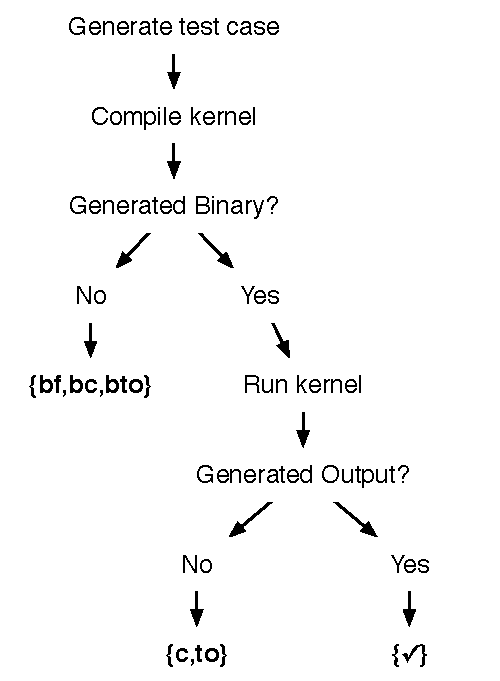
\includegraphics[width=\columnwidth]{img/test_process}%
  \caption{%
  	Test case execution, and possible outcomes. For each test case, a $(+,-)$ pair of outcomes is produced.%
  }%
  \label{fig:test-process} %
\end{figure}



\begin{enumerate}
  \item Attempt to compile sample.
  \item If compilation succeeds, generate two test payloads and execute.
\end{enumerate}

% \subsection{Parameters}
% \begin{table}[t!]
  \scriptsize %
  \centering %
  \rowcolors{2}{white}{gray!25}
  \begin{tabular}{rlll}
\toprule
 Dataset Size &   Global size &  Local size & Optimizations \\
\midrule
          256 &     (1, 1, 1) &   (1, 1, 1) &           off \\
          256 &     (1, 1, 1) &   (1, 1, 1) &            on \\
         4096 &  (128, 16, 1) &  (32, 1, 1) &           off \\
         4096 &  (128, 16, 1) &  (32, 1, 1) &            on \\
\bottomrule
\end{tabular}

  \caption{Test case parameters.}
  \label{tab:cldrive-params}
\end{table}

% Table~\ref{tab:cldrive-params}. 

\subsection{Classifying test cases}

\cc{Use the results of difftest to determine whether the input sample was formed, well-typed, free from UB, etc. Plot ratio of CLgen and CLSmith outputs according to classifications (CLSmith should be all perfect).}

\begin{enumerate}
  \item Ill-formed ASCII sequence. The test case contains syntax errors preventing compilation.
  \item Well-formed program.
  \item Well-typed program.
  \item Standard-conformant OpenCL program. The program
\end{enumerate}

\subsection{Classifying test outcomes}

We select the mode output across a range of devices. Voting is used to select the oracle output.
%
\begin{enumerate}
	\item \emph{Wrong code} Program terminates gracefully, but computes a result which differs from the majority.
	\item \emph{Build failure} Online compilation of OpenCL program fails.
	\item \emph{Runtime failure} One or more OpenCL API calls return an error status during the program execution, or the program crashes.
	\item \emph{Okay} Program terminates gracefully and computes a result which agrees with the majority.
\end{enumerate}
